\chapter{Grundlagen}
\label{cha:grundlagen}

In diesem Kapitel werden die für die Entwicklung benötigten verwendeten technischen Grundlagen erläutert.

\section{REST}

REST ist eine Abkürzung für 'Representational State Transfer' (zu deutsch 'Repräsentative Zustandsübertragung') und wurde von Roy Fielding in seiner Dissertation aus dem Jahr 2000 \cite[S. 76 ff.]{rest} definiert. Es handelt sich hierbei um eine Auflistung von Eigenschaften und Anforderungen, welche durch eine REST-API erfüllt werden sollen. REST-APIs werden für viele Dienste des Internets meist unsichtbar für die Anwender für die Kommunikation zwischen informationstechnischen Systemen verwendet. In der englischen Sprache wird häufig das Adjektiv 'RESTful' für Ressourcen verwendet, welche die REST-Prinzipien anwenden (vgl. \cite[S. 277]{swdev}).

\subsection{Anwendung in der Praxis}

Heutzutage stellen viele Dienste HTTP-APIs zur Verfügung, welche als 'RESTful' bezeichnet werden können. Die Kommunikation mit den Programmierschnittstellen beschränkt sich dabei auf das HTTP- und HTTPS-Protokoll, welches ebenfalls für den Abruf von Webinhalten im Browser verwendet wird. Durch die hohe Verbreitung wird die Implementierung neuer vernetzter Applikationen für Softwareentwickler stark vereinfacht. Das ursprünglich von Tim Berners-Lee entworfene Konzept des World Wide Web als Hypermedium wird so ebenfalls unterstützt. Ein Hypermedium beschreibt eine Ansammlung von Informationen (beispielsweise Websiten, welche im Quellcode vorliegen) mit Verweisen auf andere Informationen in dieser Menge. Bei in der Beschreibungssprache HTML (Hypertext Markup Language) geschriebenem Quellcode im World Wide Web handelt es sich um Hypertext mit Verweisen auf andere Medien (beispielsweise Quellcode anderer Webseiten; Audio-, Video- oder Bilddaten). 

Der Zugriff auf HTTP-APIs erfolgt analog zum Zugriff auf Webseiten im Internet. Je nach Anforderung werden die HTTP-Methoden 'GET', 'POST' und weitere verwendet (vgl. \cite[S. 279]{swdev}). Die von der HTTP-API beziehbaren Informationen werden mit der URL (Uniform Resource Locator) lokalisiert und angefordert. Zusätzlich können Informationen über Header (Kopfzeilen) und Cookies ausgetauscht werden, um beispielsweise Zustandsinformationen (Status des Warenkorbs in einem Webshop, Identifikationsnummer des angemeldeten Benutzers) austauschen zu können.

\begin{lstlisting}[caption={Beispiel eines Aufrufs der Graylog REST-API.}, label=bsp-rest-api, xleftmargin=6mm]
GET http://10.10.12.1:9000/api/cluster

{
  "12ac8e44-0c59-4c38-bd5e-4fe247a55893": {
    "facility": "graylog-server",
    "codename": "Noir",
    "node_id": "12ac8e44-0c59-4c38-bd5e-4fe247a55893",
    "cluster_id": "8421ad08-fe62-4a04-8576-a81cab1a9c55",
    "version": "4.3.6+36120cf",
    "started_at": "2022-09-10T23:15:05.435Z",
    "hostname": "graylog.home.arpa",
    "lifecycle": "running",
    "lb_status": "alive",
    "timezone": "Europe/Berlin",
    "operating_system": "Linux 5.4.0-125-generic",
    "is_processing": true
  }
}
\end{lstlisting}

Die Antwort der HTTP-API erfolgt in vielen Fällen maschinenlesbar in der Sprache JSON (vgl. \cite[S. 281]{swdev}).

\section{Telegram Messenger}

Der Dienst Telegram bietet seinen Nutzern eine Möglichkeit um kostenlos miteinander u.A. über Apps für die Mobilbetriebssysteme Android und iOS zu kommunizieren. Telegram hatte nach nach eigenen Angaben weltweit im Juni 2022 erstmals über 700 Millionen monatliche Nutzer und befand sich unter den fünf Apps mit den höchsten Downloadzahlen\footnote{\url{https://telegram.org/blog/700-million-and-premium}}. Der Dienst stellt damit eine beliebte Alternative zu anderen Messengern wie WhatsApp oder Signal dar. Ein Alleinstellungsmerkmal von Telegram gegenüber Whatsapp oder Signal sind die Bots und die dazugehörige API.

\subsection{Bots}

Der Begriff Bot stammt von dem englischen Begriff robot ab und bezeichnet ein Programm, welche einfache und wiederkehrende Aufgaben selbstständig erledigt. Bots werden heutzutage an vielen Stellen beim Kontakt von Menschen und informationstechnischen Systemen eingesetzt, beispielsweise in Telefonwarteschleifen oder in Webshops in Form von virtuellen Beratern für den Verkauf oder den Service. Der Telegram Messenger bietet Softwareentwicklern die Möglichkeit, mittels einer HTTP-API einen Bot auf vielfältige Weise an eigene Software anzubinden. Der Bot agiert Benutzern auf der Telegram Plattform gegenüber wie ein normaler Verbindungspartner mit dem Unterschied, dass dieser zuerst mit einer Initialnachricht ('/start') vom Benutzer aktiviert werden muss. So wird verhindert, dass  Benutzer ohne Zustimmung kontaktiert werden können. Bots können ebenfalls zu Gruppen hinzugefügt werden. Dem Entwickler stehen zahlreiche und ausführlich dokumentierte API-Funktionen\footnote{\url{https://core.telegram.org/bots/api\#available-methods}} zur Verfügung, sodass die vom Bot ausgehende Kommunikation nicht auf Textnachrichten limitiert ist. Bots stehen u.A. folgende Möglichkeiten zur Verfügung:

\begin{itemize}
\item Senden und Empfangen von Audio-, Bild- und Videodateien
\item Senden und Empfangen von Sprachnachrichten
\item Senden und Empfangen von Standorten
\item Eröffnen von Umfragen in einer Gruppe
\item Abfrage von Informationen der aktiven Kommunikationspartner: Profilbild, Name, Zeitpunkt der letzten Erreichbarkeit (sofern vom Benutzer freigegeben)
\item Gruppenadministration: Setzen und Entfernen von MOTD-Nachrichten
\item Vereinfachte Bedienung durch vom Entwickler definierte Antwortmöglichkeiten, welche durch den Anwender direkt mittels Buttons gewählt werden können
\end{itemize}

Aufgrund der weitreichenden Möglichkeiten, der kostenlosen Benutzbarkeit und der auch für frequentierte Applikationen ausreichend dimensionierten Durchsatzratenbegrenzung\footnote{\url{https://core.telegram.org/bots/faq\#my-bot-is-hitting-limits-how-do-i-avoid-this}} steht eine Vielzahl von Bots für die Benutzer der Plattform zur Verfügung. Als Beispiele seien genannt der Bot "WDR aktuell" <\lstinline{@WDRaktuell_bot}> für den Abruf von regionalen Informationen in Nordrhein-Westfalen, der von Google angebotene und daher als "verifiziert"\footnote{\url{https://telegram.org/verify}} markierte "Gmail Bot" <\lstinline{@GmailBot}> für den Nachrichtenabruf und das Senden von Antworten für Gmail sowie der Bot IFTTT <\lstinline{@IFTTT}>, welcher ebenfalls als "verifiziert" markiert wurde, da dieser vom Entwickler des Dienstes für Automatisierung und Verknüpfungen von Webanwendungen IFTTT ("if this then that") bereitgestellt wurde.

\begin{figure}[h!]
\centering
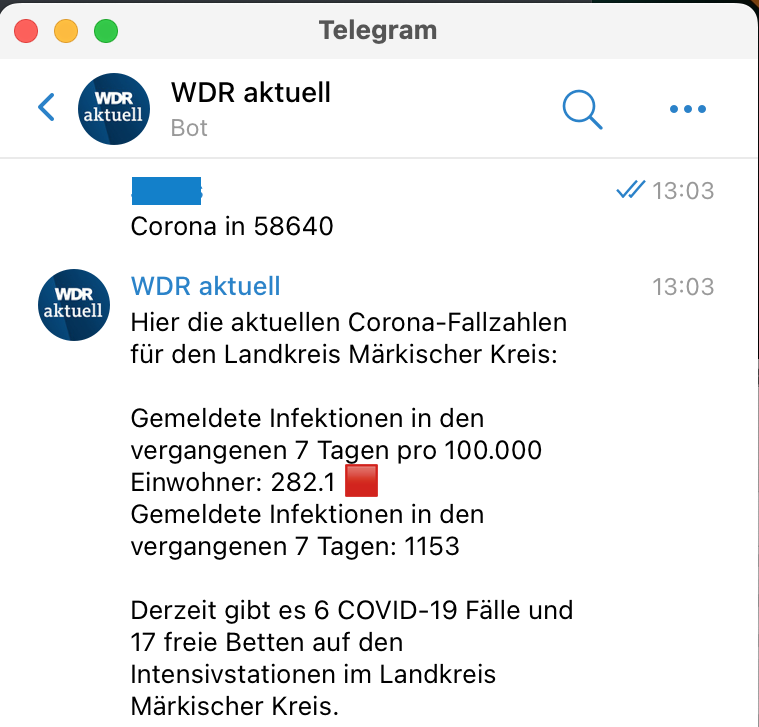
\includegraphics[scale=0.7]{telegram-bot-beispiel}
\caption{Interaktion mit dem Bot von WDR aktuell in Telegram für macOS.}
\end{figure}

\begin{figure}[h!]
\centering
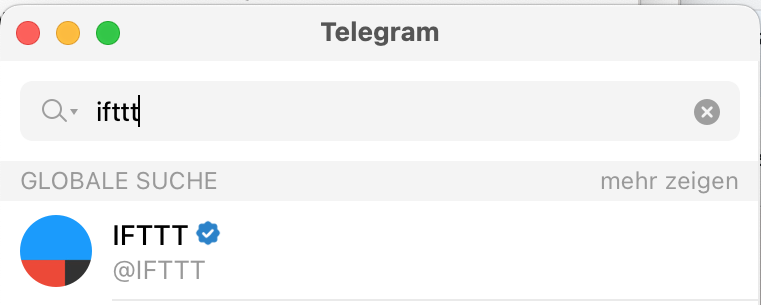
\includegraphics[scale=0.7]{verified_ifttt_bot}
\caption{Verifizierter IFTTT-Bot in der Suche von Telegram für macOS.}
\end{figure}

\subsubsection{Beziehen von Aktualisierungen von der Telegram API}
\label{sec:telegram-getting-updates}

Laut der technischen Dokumentation der Telegram API\footnote{\url{https://core.telegram.org/bots/api\#getting-updates}} stehen zwei Möglichkeiten zur Verfügung, um Aktualisierungen zu erhalten: 'long-polling' der API-Methode \lstinline{getUpdates()} oder die Verwendung eines 'webhooks'. Die beiden Möglichkeiten verwenden unterschiedliche Konzepte und bieten damit verschiedene Vor- und Nachteile. Im Fachbereich der Informatik steht der Begriff 'polling' für eine dauerhafte wiederkehrende Abfrage von Informationen bei einem Dienst. Diese Technik beansprucht viel CPU-Zeit eines Systems und wird aufgrund des geringen Gegenwerts der meist leer ausgehenden Abfragen als teuer bezeichnet. 'long-polling' beschreibt eine Technik, bei welcher der Client einer HTTP-Abfrage einen verlängerten Zeitraum bis zum Erhalt der Antwort vom Server akzeptiert, ohne die Abfrage aufgrund einer Zeitüberschreitung abzubrechen. Die Länge des Zeitraums ist variabel. 'long-polling' bietet damit gegenüber dem klassischen 'polling' den Vorteil, dass die benötigte Rechenzeit durch die verlängerten Abfragezeiträume stark reduziert wird. Die Software- und Betriebssystementwicklung bietet eine Technik, um die Verwendung von teurem 'polling' zu umgehen: die Verwendung von 'interrupts' oder 'callbacks' (zu deutsch "Rückruf"). Hierbei erhält der Absender der Anfrage eine Rückmeldung, sobald die Antwort vorliegt. Der Vorteil dieser Technik ist, dass nach dem Absenden der Anfrage keine CPU-Zeit seitens des Absenders notwendig ist. Es muss jedoch eine Möglichkeit vorhanden sein, den Absender im Falle einer eingehenden Antwort zum Vorgang zurückzuführen, sodass die weitere Bearbeitung möglich wird. Im Falle der Anbindung der Telegram API übernimmt dies der 'webhook'. Der 'webhook' muss (durch die Telegram-API) öffentlich aus dem Internet erreichbar und durch den Verwalter des Bots im Vorhinein durch eine entsprechenden URL definiert worden sein. Wird eine Nachricht an den Bot gesendet, prüft die Telegram-API, intern, ob Definitionen für webhooks vorliegen. Im positiven Fall sendet die Telegram API eine HTTP-Anfrage an die URL des webhooks mit den Details zur eingegangenen Nachricht. Nach Erhalt der Anfrage durch den webhook muss dieser die Daten zur verarbeitenden Software zurückführen und die weitere Bearbeitung auslösen.

\subsubsection{Erstellung eines Bots}

Um ein Programm über die Telegram Bot-API anbinden zu können, muss zuvor ein Bot über Telegram erstellt werden. Hierzu wird der Bot \lstinline{@BotFather} verwendet. Sämtliche Einstellungen zu Bots werden über \lstinline{@BotFather} vorgenommen. Soll ein neuer Bot erstellt werden, werden die benötigten Informationen abgefragt. Nachdem der Anzeigename und der Benutzername festgelegt werden, erhält der Benutzer die Zugangsdaten für die HTTP-API und der Bot ist einsatzbereit. \lstinline{@BotFather} kann jederzeit erneut kontaktiert werden, um weitere Einstellungen vorzunehmen: es können Profilbild und Beschreibung geändert, sowie vordefinierte Kommandos festgelegt werden. Der Zugriff auf die HTTP-API erfolgt über die Basis-URL \lstinline{https://api.telegram.org/bot<token>/METHOD_NAME}\footnote{\url{https://core.telegram.org/bots/api\#making-requests}}, wobei \lstinline{<token>} der von \lstinline{@BotFather} erhaltene Zugriffsschlüssel und \lstinline{METHOD_NAME} die API-Methode (beispielsweise \lstinline{getUpdates} oder \lstinline{sendMessage}) ist. Weitere laut API-Dokumentation benötigte Parameter werden als Parameter der HTTP-Anfragen vom Typ 'GET' oder 'POST' übermittelt. Die Antwort der API erfolgt in Form eines JSON-Objekts.

\begin{lstlisting}[caption={Beispiel eines Aufrufs der Telegram HTTP-API. Erhalt einer Textnachricht "Hallo Welt".}, label=lst:bsp-telegram-api, xleftmargin=6mm]
GET https://api.telegram.org/bot123456:ABC-DEF1234ghIkl-zyx57W2v1u123ew11/getUpdates

{
    "ok": true,
    "result": [
        {
            "update_id": 987654321,
            "message": {
                "message_id": 626,
                "from": {
                    "id": 12345678,
                    "is_bot": false,
                    "first_name": "Jonas",
                    "username": "-entfernt-",
                    "language_code": "de"
                },
                "chat": {
                    "id": 12345678,
                    "first_name": "Jonas",
                    "username": "-entfernt-",
                    "type": "private"
                },
                "date": 1662808990,
                "text": "Hallo Welt"
            }
        }
    ]
}
\end{lstlisting}

\section{Graylog Open}

Graylog Open ist ein Softwareprodukt der Firma Graylog, Inc mit dem Hauptsitz in Houston, Texas in den USA. Das Produkt stellt eine kompakte Verwaltungsoberfläche für die Erfassung von Systemprotokollen bereit, welche in einer ElasticSearch Suchmaschine vorgehalten werden. Der Quellcode der Software kann öffentlich eingesehen werden\footnote{\url{https://github.com/Graylog2/graylog2-server}}. Hohe Anforderungen an die (Ausfall-)sicherheit moderner und komplexer IT-Systeme führen zu der Notwendigkeit, die Funktionsfähigkeit der Systeme möglichst allumfassend und automatisiert zu prüfen. Herkömmliche Monitoringsysteme mit einem Fokus auf die Erreichbarkeit oder die Überwachung von vordefinierten Fehlerausgaben erfüllen diese Anforderungen nicht. Fehlerzustände sollen in Echtzeit, möglichst vor und spätestens zum Zeitpunkt einer durch den Anwender spürbaren Einschränkung auffallen. Informationstechnische Systeme in sämtlichen Bereichen sind längst zu komplex geworden, um alle Fehlerquellen im Vorhinein bestimmen und gezielt überwachen zu können. Aus diesem Grund wird ein anderer Ansatz als beim herkömmlichen Monitoring angewendet: die Erfassung der Systemprotokolle der zu überwachenden Systeme. Diese ermöglichen einen umfassenderen Blick auf die aktuellen Ereignisse. Durch die Anwendungsprotokolle können Fehlerzustände eines Webservers beispielsweise bereits nach dem ersten Besuch eines Besuchers einer durch den fehlerhaften Webserver beeinträchtigten Webseite erkannt werden.

\subsection{Erfassung von Systemprotokollen}

Graylog Open ist kompatibel zu einer Vielzahl heutiger Betriebssysteme und Anwendungen. Linuxbasierte Systeme verwenden häufig einen Dienst zur zentralen und systemweiten Erfassung der Anwendungsprotokolle, welcher das in RFC 3164 standardisierte Protokoll 'syslog'\footnote{\url{https://www.ietf.org/rfc/rfc3164.txt}} verwendet. Dieser schreibt in der Standardkonfiguration vieler aktueller Betriebssysteme auf Basis des Linux Derivats Debian alle Meldungen in Textform in die Datei \lstinline{/var/log/syslog}, bei Systemen auf Basis des Derivats RedHat Enterprise Linux in die Datei \lstinline{/var/log/messages}. Die Position dieser Ausgabedatei auf dem Dateisystem ist für die Verarbeitung der Meldungen in Graylog jedoch nicht wichtig, da die Meldungen nach einer Anpassung der Konfiguration des Dienstes (offiziell wird nur die Software 'rsyslog' und 'syslog-ng' von Graylog unterstützt\footnote{\url{https://docs.graylog.org/docs/syslog}}) über das Netzwerk per UDP und optionaler TLS-Verschlüsselung an Graylog übertragen werden. In Graylog muss hierzu die Annahme von Daten über das Netzwerk mit dem syslog-Protokoll aktiviert werden. Mittels einer Input-Konfiguration wird ein Port an der zum überwachenden System nächstgelegenen Netzwerkschnittstelle eröffnet, auf welchem die Software auf eintreffende Meldungen im syslog-Format lauscht.

Auch mit Docker bereitgestellte Microservices können global überwacht werden, ohne die Konfiguration der Container oder sogar die der Anwendungen in einem gestarteten Container einzeln anpassen zu müssen. Hierzu wird nicht das syslog-Protokoll, sondern das von Docker ohnehin unterstützte\footnote{\url{https://docs.docker.com/config/containers/logging/gelf/}} Protokoll GELF verwendet. Es ist ebenfalls eine zentrale Änderung der Konfiguration des Docker-Dienstes notwendig, um fortan die Protokolle aller neu gestarteten Container über das wahlweise UDP- oder TCP-basierte GELF-Protokoll an die Graylog-Instanz zu senden. Die an Graylog übertragenen Daten entsprechen der Ausgabe des \lstinline{docker logs} Kommandos. Um den Empfang von Daten über das GELF-Protokoll seitens Graylog zu ermöglichen, ist es analog zur Einrichtung für das syslog-Protokoll notwendig, mittels einer Input-Konfiguration einen Port auf einer Netzwerkschnittstelle zu reservieren.

Systemprotokolle aus Windows können nicht direkt verarbeitet werden. Es ist der Einsatz einer Middleware wie Winlogbeat notwendig, welche die Protokolle auf dem System erfasst und die Daten über ein Netzwerkprotokoll an Graylog sendet.\footnote{\url{https://docs.graylog.org/docs/windows}}

\subsection{Verarbeitung}

Für die Verarbeitung der erfassten Daten stellt Graylog dem Systemadministrator eine Vielzahl von Möglichkeiten zur Verfügung, welche aufgrund der Fokussierung der Abschlussarbeit auf die Implementierung eines Bots für die Informationsabfrage aus Graylog mittels der angebotenen REST-API nur bezogen auf das Ziel der Abschlussarbeit erläutert werden. Nach der Erfassung der Daten über die konfigurierten Input-Kanäle werden diese in einer Elasticsearch Suchmaschine hinterlegt und nach vom Administrator definierten Filterausdrücken durchsucht. Schließlich sind die erfassten Nachrichten über die Weboberfläche durchsuchbar. Für die Suche wird eine an Apache Lucene (Programmbibliothek für Volltextsuche) angelehnte Syntax verwendet. Der Administrator kann Informationen mittels regulären Ausdrücken aus eingehenden Nachrichten extrahieren und die Graylog-Instanz so auf die zu überwachenden Applikationen anpassen. Beispielsweise kann der HTTP Statuscode eines Eintrags von einem Webserver extrahiert werden:

\begin{figure}[h!]
\centering
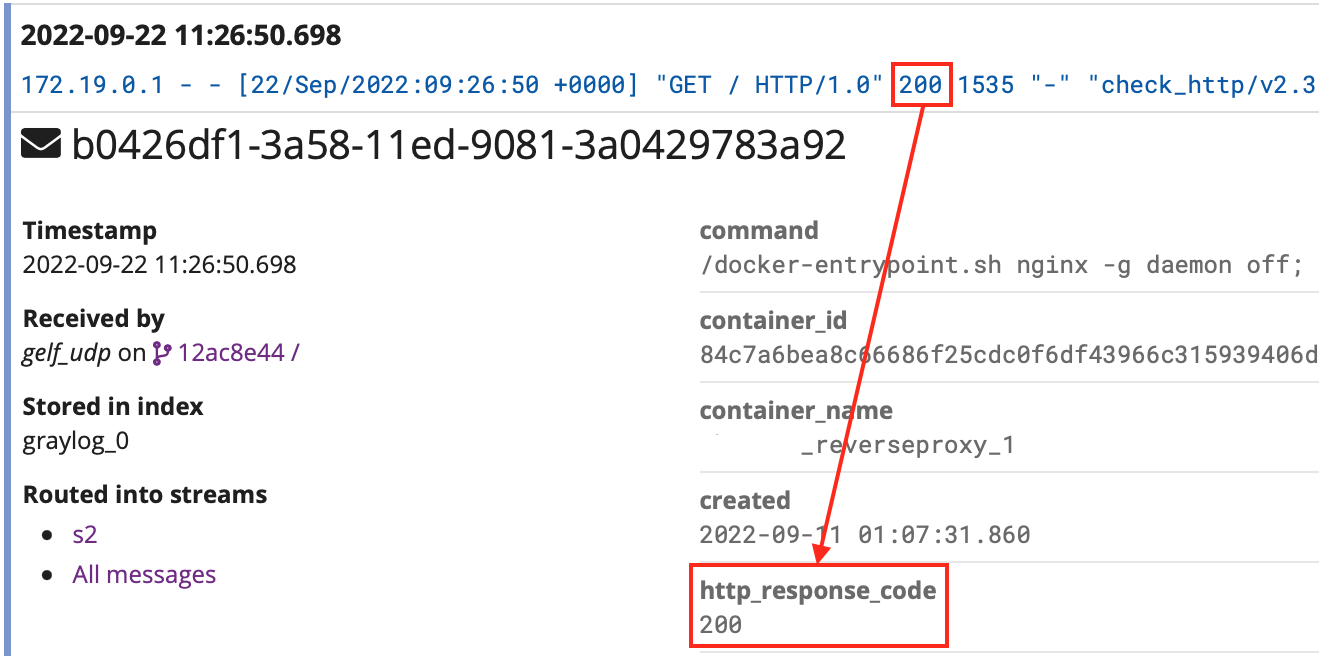
\includegraphics[scale=0.7]{graylog-bsp-msg}
\caption{Extrahieren von Daten aus eingehenden Meldungen in Graylog.}
\end{figure}

\subsection{Zugriff per API}

Graylog stellt eine REST-API zur Verfügung, auf welche sowohl mit der integrierten Webschnittstelle als auch per Fernzugriff zugegriffen werden kann. Die integrierte Webschnittstelle nutzt die API für das Beziehen der Informationen aus der ElasticSearch Suchmaschine. Jede Graylog-Instanz verfügt standardmäßig über eine auf der API-Dokumentationssoftware Swagger basierende Übersicht der verfügbaren Funktionen. Die Oberfläche ermöglicht es zusätzlich, die API-Funktionen aus dem Browser heraus mit selbstgewählten Parametern aufzurufen. Softwareentwickler erhalten so eine Übersicht über die in der installierten Graylog-Version verfügbaren API-Funktionen. Das prüfen von API-Funktionen mit Drittanbieterprogrammen wie curl oder Postman entfällt.

\section{Amazon Web Services}

Der Cloudanbieter AWS ist ein Tochterunternehmen des US-amerikanischen Versandhändlers Amazon. Das Unternehmen bietet seine Dienste vor allem für professionelle Endanwender und Unternehmen an. AWS bietet eine Vielzahl von Diensten, welche 'on-demand' (zu deutsch 'auf Abruf') verfügbar sind nach dem Prinzip 'pay as you go' (zu deutsch 'abgerechnet nach Verbrauch') berechnet werden. Zu den bekanntesten Diensten zählen EC2 (elastic compute cloud), welcher virtuelle Maschinen bereitstellt sowie S3 (simple storage service), für das Buchen von Speicherkapazität. AWS gehört neben den allesamt US-amerikanischen Anbietern Microsoft Azure, Google Cloud, Oracle Cloud sowie dem chinesischen Anbieter Alibaba Cloud laut dem Anbieter für Marktforschungsergebnisse Gartner zu den führenden Cloudanbietern weltweit\footnote{\url{https://www.gartner.com/technology/media-products/reprints/AWS/1-271W1OSP-DEU.html}}. Derzeit gibt es keinen gleichwertigen Anbieter aus Europa. Die Anbieter IONOS und Strato aus Deutschland sowie OVH aus Frankreich bieten nur einen Bruchteil der Umfänge der Konkurrenten an.

AWS betreibt zahlreiche Rechenzentren weltweit und stellt einen Großteil der Dienste an allen Standorten zur Verfügung. Zahlreiche Dienste lassen sich über die Webschnittstelle 'AWS Konsole' verwalten. Als 'on-demand' Anbieter steht für sämtliche Dienste auch die Bedienung über eine API-Softwareschnittstelle zur Verfügung, sodass Ressourcen bei Bedarf von Programmen selbstständig gebucht und vollständig verwaltet werden können. Die Abrechnung variiert je nach Dienst. Rechenressourcen werden nach Stunden oder Minuten abgerechnet, Speicherressourcen nach Datenmenge und auftragsbasierte Dienste (vgl. \autoref{sec:amazon-transcribe}) nach Auftragskontingenten. AWS bietet zusätzlich ein freies Kontingent an. Die anfallenden Kosten lassen sich im Vorhinein mit dem AWS Pricing Calculator\footnote{\url{https://calculator.aws/}} bestimmen. 

Für die Verwendung der AWS API mit der Programmiersprache Python stellt ein Entwicklerteam das offizielle SDK (engl. Abkürzung für 'software development kit', zu deutsch "Sammlung von Werkzeugen für die Programmentwicklung") unter dem Namen boto3 zur Verfügung. Das SDK erleichtert die Bedienung der verschiedenen API-Funktionen in Verbindung mit den zugrundeliegenden Paradigmen der verwendeten Programmiersprache. Es wird mit abstrakten Python-Objekten gearbeitet, die Verarbeitung von HTTP-Anfragen (beispielsweise mit der Programmbibliothek 'requests') ist damit nicht mehr notwendig. Das SDK übernimmt weiterhin die Authentifizierung gegenüber der API.

\subsection{Amazon Transcribe}
\label{sec:amazon-transcribe}

Mit dem Dienst Amazon Transcribe können Audiodateien zu Text mittels künstlicher Intelligenz transkribiert werden. Der Dienst unterstützt mehrere Sprachen und Dialekte. Standardmäßig wird ein allgemeines Sprachmodell des Anbieters verwendet. Es ist ebenfalls möglich, ein eigenes Sprachmodell zu trainieren und importieren. Bei der Bedienung über die AWS Konsole muss ein URI zu einer Audiodatei in einem S3-Speicher angegeben werden. Der Dienst hinterlegt den Text in einer Datei ebenfalls in einem S3-Speicher, optional kann dabei der Quellspeicher eingestellt werden. Eine Übersetzung in Echtzeit ist nicht möglich. Das Limit für gleichzeitige Vorgänge pro Benutzer liegt bei 100. Neue Aufträge können so lange nicht eingereicht werden, bis die Anzahl wieder unter dem Limit liegt. Bei einer absehbaren Überschreitung des Limits kann eine Auftragswarteschlange verwendet werden, um die Aufträge zuzuführen. Die Abrechnung erfolgt außerhalb des freien Kontingents nach Zeitkontingenten und beginnt bei 0,024 USD pro angefangene Minute.

\subsection{Amazon Polly}
Polly ist ein TTS-Dienst ('text-to-speech', zu deutsch 'Text zu Sprache') und bildet das Gegenstück zu Amazon Transcribe. Der Dienst unterstützt ebenfalls verschiedene Sprachen und Dialekte. Je nach Sprache können verschiedene Modelle verwendet werden, welche verschiedene Persönlichkeiten und Geschlechter darstellen. Dabei wird zwischen den Typen 'standard' und 'neural' unterschieden. 'neural'-Modelle erzeugen eine gegenüber des Typs 'standard' optimierte Ausgabe, welche der menschlichen Aussprache so ähnlich wie möglich kommen soll. Die Abrechnung erfolgt außerhalb des freien Kontingents nach Zeichenkontingenten und beginnt bei 4 USD für eine Million Zeichen. Der Typ 'neural' kostet bei gleicher Verwendung etwa das Vierfache. 
